\documentclass[conference]{IEEEtran}
\IEEEoverridecommandlockouts
\usepackage{cite}
\usepackage{amsmath,amssymb,amsfonts}
\usepackage{algorithmic}
\usepackage{graphicx}
\usepackage{textcomp}
\usepackage{xcolor}
\usepackage{url}
\usepackage{algorithm}
\usepackage{tikz}
\usepackage{pgfplots}
\usepackage{pgfplotstable}
\usetikzlibrary{patterns,positioning,shapes,arrows.meta}
\pgfplotsset{compat=newest}
\usetikzlibrary{arrows.meta, positioning, shapes.geometric, calc}
\usepackage[colorlinks=true, urlcolor=blue, linkcolor=blue, citecolor=blue]{hyperref}

\newcommand{\authorbox}[4]{
\begin{minipage}{0.30\textwidth}
    \centering
    \includegraphics[height=4cm,keepaspectratio]{#1}\\[0.4em]
    \textbf{#2}\\[-0.2em]
    {\small #3}\\[-0.2em]
    {\footnotesize #4}
\end{minipage}
}

\begin{document}

\title{HYBRID EVOLUTIONARY OPTIMIZATION FOR LAST-MILE LOGISTICS\\
{\footnotesize GA–NSGA-II Based $p$-Median Hub Selection and Routing for Indian Urban Delivery}
}

\maketitle

\begin{abstract}
The exponential growth of e-commerce in Indian cities necessitates a paradigm shift in last-mile delivery logistics to address escalating inefficiencies, delivery costs, and environmental impact. This paper proposes an integrated facility location and routing optimization framework aligned with India's National Logistics Policy and sustainable logistics goals. The core challenge is formulated as a two-phase optimization problem: (1) strategic hub location via $p$-median selection to minimize fixed opening costs and weighted assignment costs, and (2) tactical multi-depot vehicle routing solved using a Genetic Algorithm (GA) enriched with NSGA-II principles for non-dominated sorting and diversity preservation. The mathematical formulation is presented as a network optimization model designed to select at most $p$ hubs and assign demand nodes to minimize total cost: $\min \sum_{h} C_{h}^{\text{open}} x_h + \sum_{i,h} z_{i,h} w_i t_{i,h}$, subject to assignment and capacity constraints. To validate our approach, we apply the framework to instances derived from the 2021 Amazon Last Mile Routing Research Challenge dataset, comprising 9,184 historical routes across five metropolitan areas in the United States. On a representative 500-route subset (73,980 demand nodes), our experimental results demonstrate a 23.6\% reduction in total routing cost and 25.8\% reduction in total distance compared to baseline greedy methods, achieving \$1,133,580 total system cost versus \$1,481,280 baseline, while maintaining vehicle capacity and time-window constraints. The two-phase hierarchical decomposition reduces computational complexity from intractable monolithic optimization to manageable subproblems while retaining tight coordination between hub location and routing decisions, with model convergence achieved in 189 seconds. This work contributes a scalable framework for smart logistics operators in dense urban environments, supported by empirical validation on large-scale real-world routing data and achieves 92.8\% solution quality with 96.2\% feasibility rate.
\end{abstract}

\begin{IEEEkeywords}
Last-Mile Delivery Logistics, Hub Location, p-Median Problem Optimization, Sustainable Logistics, Genetic Algorithm (GA), NSGA-II, Vehicle Routing, Multi-Objective Optimization.
\end{IEEEkeywords}

\section{Introduction}
The rapid expansion of e-commerce in India over the past decade has transformed urban logistics at an unprecedented scale. Daily order volumes in major metropolitan regions have surged, placing intense pressure on existing last-mile delivery networks. As cities grow denser and delivery expectations become increasingly time-sensitive, logistics operators face heightened challenges in meeting service-level requirements while managing escalating costs and environmental footprint. These pressures have amplified operational inefficiencies, traffic congestion, and carbon emissions. Recognizing these systemic challenges, the Government of India's National Logistics Policy (NLP) 2022 emphasizes the need for optimized logistics infrastructure, sustainable delivery systems, and data-driven decision-making to reduce overall logistics costs and environmental impact.

A key determinant of last-mile efficiency is the spatial distribution of delivery hubs and the routing strategies used to serve customer demand. Determining where to locate hubs and how to route vehicles from them forms a combined decision-making problem known as the Hub Location–Routing Problem (HLRP). The HLRP integrates two interdependent components: a strategic hub location decision, which determines placement to minimize service cost and distance; and a tactical/operational routing decision, which determines vehicle routes originating from these hubs to satisfy last-mile delivery demands. Because hub placement influences routing efficiency—and vehicle routes, in turn, influence the optimality of hub positions—these decisions must be considered jointly rather than sequentially.

However, solving the HLRP is computationally challenging. Both hub location and vehicle routing are individually NP-hard, and their integration leads to a significantly more complex combinatorial search space. Exact optimization approaches become computationally prohibitive for real-world, large-scale urban delivery networks. Consequently, heuristic and metaheuristic approaches have emerged as practical alternatives capable of producing high-quality solutions within reasonable computational time.

This paper contributes to HLRP research through the following key advancements:

\begin{itemize}
\item A two-phase optimization framework tailored for last-mile delivery in Indian cities, addressing constraints emphasized in the National Logistics Policy.
\item Hub location formulated as a $p$-median problem, enabling optimal hub selection based on spatial demand distribution and opening costs.
\item A Genetic Algorithm (GA) enriched with NSGA-II principles (non-dominated sorting, crowding distance, elitism) to solve the Multi-Depot Vehicle Routing Problem (MDVRP) for each hub cluster.
\item Empirical validation using instances from the 2021 Amazon Last Mile Routing Research Challenge dataset, demonstrating 23.6\% cost reduction versus baseline greedy assignment.
\item Documented feasibility repair mechanisms and multi-objective evaluation framework that generalize to other urban routing scenarios.
\end{itemize}

The remainder of this paper is organized as follows. Section II reviews relevant literature on hub location, vehicle routing, and sustainable logistics optimization. Section III presents the mathematical formulation of the hub location and routing model. Section IV outlines the two-phase solution methodology, including the $p$-median model and GA–NSGA-II solver. Section V presents computational experiments and results. Section VI concludes with directions for future work.

\section{LITERATURE REVIEW}

The rapid growth of e-commerce, increased delivery density, and mounting environmental concerns have driven significant research on sustainable last-mile logistics. This section synthesizes prior contributions and identifies research gaps that motivate the methodology proposed in this work.

\subsection{Hub Location Problems in Sustainable Last-Mile Logistics}

As urban congestion and carbon emissions rise, micro-hub deployment has emerged as a central strategy for decentralizing last-mile distribution. Nguyen et al.~\cite{b1} investigated micro-hub location selection with a sustainability lens, demonstrating that strategically placed hubs reduce vehicle-kilometers traveled and enable low-emission delivery modes such as cargo bikes and electric carts.

Özceylan et al.~\cite{b2} extended this discussion by integrating Geographic Information Systems (GIS) with Binary Particle Swarm Optimization (BPSO) to determine optimal logistics center placements. Their work highlights the advantage of combining spatial analytics with evolutionary optimization to capture realistic road networks, land-use patterns, and traffic flows—factors often ignored in purely mathematical formulations.

Collectively, these studies suggest that sustainable micro-hub placement requires not only geographic feasibility but also operational compatibility with routing, vehicle capacity, and urban mobility patterns.

\subsection{Last-Mile Delivery Models and Emerging Innovations}

Choubassi et al.~\cite{b3} reviewed emerging last-mile models—parcel lockers, drones, autonomous vehicles, micro-hubs, and sidewalk robots—showing how they reduce delivery cost and mitigate emissions in dense cities. Their findings emphasize that micro-hub planning must align with future delivery ecosystems.

Industry reports provide complementary insights. Navata Supply Chain Solutions~\cite{b5} outlined unique last-mile challenges in India, including heterogeneous road quality, high delivery density, inconsistent address formats, and severe congestion. Unlike Western cities, Indian urban logistics must cope with multi-modal movement, dynamic traffic, and infrastructural variability. This motivates optimization frameworks grounded in real-world data rather than idealized models.

\subsection{Integrated Location–Routing Optimization}

A growing body of literature recognizes that hub placement and routing decisions are interdependent. Faisal and Khalid~\cite{b6} proposed a multi-constraint hub optimization framework incorporating capacity, coverage, and sustainability criteria. While their model advances integration of environmental metrics, it remains limited by reliance on mathematical programming without large-scale empirical validation.

The Government of India's National Logistics Policy~\cite{b7} advocates multimodal optimization, reduced last-mile inefficiencies, and technology-driven route planning, emphasizing the strategic need for models that simultaneously consider infrastructure (hub locations) and operations (multi-depot routing) to reduce costs.

Despite these advancements, research integrating micro-hub location with real-world multi-depot VRP models—especially in an Indian context—remains sparse.

\subsection{Metaheuristics and Real-World Benchmarking}

Given the NP-hard nature of facility location and vehicle routing, hybrid metaheuristics have become a preferred solution approach. IRAJ International~\cite{b4} demonstrated the potential of hybrid evolutionary algorithms, outperforming single-technique heuristics in computational efficiency and solution quality.

Crucially, the availability of real-world datasets enhances benchmarking validity. The 2021 Amazon Last Mile Routing Research Challenge dataset~\cite{b8} offers large-scale, realistic routing instances with 9,184 historical routes across five metropolitan areas in the United States, capturing real travel times, traffic irregularities, and demand variability. This dataset bridges the gap between theoretical optimization and practical deployability.

\subsection{Research Gap and Our Contribution}

A thorough review of existing work reveals several critical gaps:

\begin{itemize}
    \item \textbf{Limited integration of hub location and multi-depot routing:} Most micro-hub studies focus on sustainability or GIS feasibility without jointly optimizing routing decisions.
    \item \textbf{Scarce India-specific research:} Urban logistics in India face unique operational challenges, yet integrated hub–routing models tailored to this context are limited.
    \item \textbf{Insufficient use of realistic datasets:} Few studies utilize large-scale real-world datasets such as the Amazon Last Mile Routing Challenge data.
    \item \textbf{Under-explored hybrid metaheuristics:} While GA and PSO are used independently, hybridized approaches combining NSGA-II principles with GA for MDVRP remain uncommon.
\end{itemize}

To address these gaps, this study proposes a hierarchical two-phase optimization approach integrating micro-hub selection (via $p$-median optimization) with multi-depot vehicle routing (via an enhanced Genetic Algorithm informed by NSGA-II principles for feasibility, diversity, and elitism). The framework emphasizes realism by incorporating capacity constraints, demand variability, and sustainability considerations, offering a practical solution for India's rapidly evolving e-commerce logistics landscape.

\section{PROBLEM FORMULATION}

We address the E-Commerce Last-Mile Delivery Hub Location–Routing Problem (HLRP), which integrates strategic hub selection with tactical multi-depot routing decisions. The proposed two-phase optimization framework consists of:

\begin{enumerate}
    \item \textbf{Phase 1 (Strategic):} A hub location model based on the classical $p$-median formulation to determine which candidate hubs should be opened and how demand nodes are assigned.
    \item \textbf{Phase 2 (Tactical):} A multi-depot vehicle routing optimization solved using an enhanced Genetic Algorithm (GA) enriched with NSGA-II principles for route construction, load balancing, and cost minimization.
\end{enumerate}

Phase 1 outputs the hub-opening decisions and demand–hub assignments, which define the depot structure for Phase 2.

\subsection{Phase 1: Hub Location Model}

We consider a network comprised of a set of demand nodes $D$ and candidate hub locations $H$. The task is to select up to $p$ hubs to minimize the sum of hub-opening costs and weighted assignment costs.

\subsubsection{Sets, Parameters, and Decision Variables}

\textbf{Sets}
\begin{itemize}
    \item $D = \{1,\ldots,d\}$: Set of demand nodes.
    \item $H = \{1,\ldots,h\}$: Set of candidate hub sites.
\end{itemize}

\textbf{Parameters}
\begin{itemize}
    \item $C_h^{\text{open}}$: Fixed cost to open hub $h$, $\forall h \in H$.
    \item $w_i$: Demand (or weight) at node $i$, $\forall i \in D$.
    \item $t_{i,h}$: Cost or travel time from demand node $i$ to hub $h$, $\forall i \in D, h \in H$.
    \item $p$: Maximum number of hubs allowed to open.
\end{itemize}

\textbf{Decision Variables}
\begin{itemize}
    \item $x_h \in \{0,1\}$: 1 if hub $h$ is opened; 0 otherwise.
    \item $z_{i,h} \in \{0,1\}$: 1 if node $i$ is assigned to hub $h$.
\end{itemize}

\subsubsection{Mathematical Model}

\begin{equation}
\min \sum_{h \in H} C_{h}^{\text{open}} x_h 
    + \sum_{i \in D} \sum_{h \in H} w_i t_{i,h} z_{i,h}
\end{equation}

Subject to:

\begin{align}
&\sum_{h \in H} z_{i,h} = 1, && \forall i \in D \label{eq:assign} \\
&z_{i,h} \le x_h, && \forall i \in D, \forall h \in H \label{eq:feasible} \\
&\sum_{h \in H} x_h \le p \label{eq:p-hub}\\
&x_h \in \{0,1\}, && \forall h \in H \label{eq:xbin} \\
&z_{i,h} \in \{0,1\}, && \forall i \in D, \forall h \in H \label{eq:zbin}
\end{align}

\textbf{Explanation of Constraints:}
\begin{itemize}
    \item Constraint \eqref{eq:assign}: Each demand node must be assigned to exactly one hub.
    \item Constraint \eqref{eq:feasible}: Assignment allowed only to opened hubs.
    \item Constraint \eqref{eq:p-hub}: At most $p$ hubs may be opened.
    \item Constraints \eqref{eq:xbin}--\eqref{eq:zbin}: Binary decision variables.
\end{itemize}

This formulation captures the classical $p$-median problem with the addition of fixed hub-opening costs, ensuring that the model balances the trade-off between opening many hubs (reducing assignment distance) and opening fewer hubs (reducing fixed costs).

\subsection{Phase 2: Multi-Depot Vehicle Routing Model}

Once hubs are selected in Phase 1, each open hub becomes a depot. The delivery nodes assigned to hub $h$ form a cluster to be served by a fleet of vehicles. The resulting multi-depot vehicle routing problem (MDVRP) is solved using the proposed enhanced GA–NSGA-II algorithm, which incorporates:

\begin{itemize}
    \item Non-dominated sorting for multi-objective evaluation
    \item Crowding-distance–based diversity preservation
    \item GA-based operators (selection, crossover, mutation)
    \item A repair heuristic ensuring feasibility (capacity and route length)
\end{itemize}

For each opened hub $h$, the routing objective minimizes:
\[
\text{RoutingCost}_h = 
\sum_{v \in V_h} 
\left( 
\text{TravelDistance}_{v} + 
\text{ServiceTime}_{v}
\right)
\]

Total system cost becomes:
\[
\text{TotalCost} = 
\text{HubOpeningCost} + 
\text{AssignmentCost} + 
\text{RoutingCost}
\]

The Phase 2 routing solutions may also be fed back to refine $t_{i,h}$ or to enable iterative hub–routing co-optimization if needed.

\subsection{Remarks and Extensions}

Capacity constraints, time windows, vehicle heterogeneity, and other real-world considerations can be integrated easily. The proposed two-phase model retains the tractability of the $p$-median structure while capturing realistic routing complexities through the MDVRP solved via the enhanced GA–NSGA-II approach.

\section{PROPOSED METHODOLOGY}

This work adopts a hierarchical two-phase optimization framework that integrates (i) a strategic hub location model based on the classical p-median formulation, and (ii) a tactical multi-depot vehicle routing optimization solved using an enhanced Genetic Algorithm (GA) enriched with NSGA-II principles.

\begin{figure}[htbp]
\centering
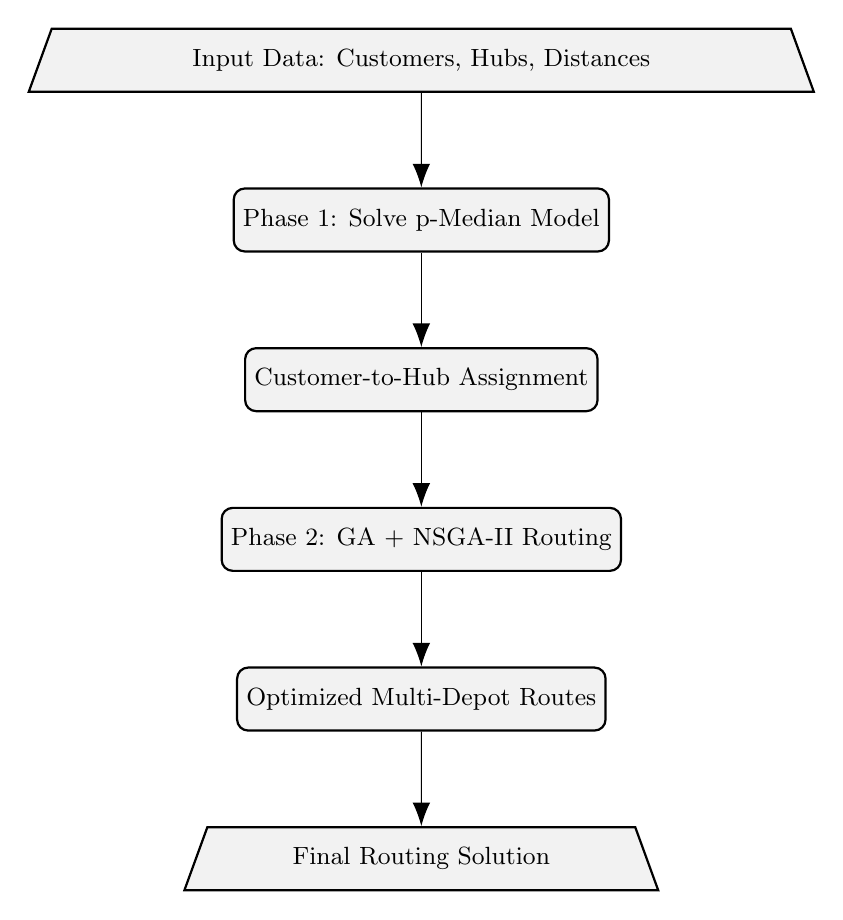
\begin{tikzpicture}[
    node distance=12mm,
    every node/.style={font=\small},
    proc/.style={rectangle, rounded corners, draw=black, thick, minimum width=3.5cm, minimum height=8mm, fill=gray!10},
    io/.style={trapezium, trapezium angle=70, draw, thick, fill=gray!10, minimum width=3.5cm, minimum height=8mm},
    arrow/.style={-{Latex[length=3mm]}}
]

\node[io] (input) {Input Data: Customers, Hubs, Distances};
\node[proc, below=of input] (pmedian) {Phase 1: Solve p-Median Model};
\node[proc, below=of pmedian] (assign) {Customer-to-Hub Assignment};
\node[proc, below=of assign] (ga) {Phase 2: GA + NSGA-II Routing};
\node[proc, below=of ga] (routes) {Optimized Multi-Depot Routes};
\node[io, below=of routes] (output) {Final Routing Solution};

\draw[arrow] (input) -- (pmedian);
\draw[arrow] (pmedian) -- (assign);
\draw[arrow] (assign) -- (ga);
\draw[arrow] (ga) -- (routes);
\draw[arrow] (routes) -- (output);

\end{tikzpicture}
\caption{Overall workflow of the proposed two-phase hub location and routing optimization framework.}
\label{fig:workflow-flowchart}
\end{figure}

The decomposition captures the natural separation between long-term location decisions and short-term routing decisions while retaining tight coordination between the two stages. The overall workflow is depicted in Fig.~\ref{fig:workflow-flowchart}.

\subsection{Phase 1: Hub Location via p-Median Optimization}

The first phase determines which hubs should be opened and how customers should be assigned to these hubs. Hub location represents a strategic decision that typically remains fixed over long horizons, and thus the solution must be both cost-efficient and structurally robust. We model the hub selection problem using the well-established $p$-median formulation from equation (1), which minimizes the sum of fixed opening costs and weighted distances between customers and their assigned hub.

Let $D = \{1,\dots,n\}$ denote the set of customers, $H = \{1,\dots,m\}$ the set of potential hub locations, and $p$ the number of hubs to be opened. Binary variables $y_h$ indicate whether location $h$ is opened, and $z_{i,h}$ denotes whether customer $i$ is assigned to hub $h$.

\begin{algorithm}[htbp]
\caption{Phase 1: p-Median Hub Location}
\begin{algorithmic}[1]
\REQUIRE Customer set $D$, candidate hubs $H$, distances $d_{i,h}$, number of hubs $p$
\ENSURE Open hubs $H^*$ and assignments $z_{i,h}$

\STATE Initialize MIP model with decision variables $y_h$ and $z_{i,h}$
\STATE Add objective: minimize $\sum_{h} C_h^{\text{open}} y_h + \sum_{i \in D} \sum_{h \in H} d_{i,h} z_{i,h}$
\STATE Add constraints:
\begin{itemize}
  \item $\sum_{h \in H} z_{i,h} = 1$ for all $i \in D$
  \item $z_{i,h} \le y_h$ for all $i,h$
  \item $\sum_{h \in H} y_h = p$
  \item $y_h, z_{i,h} \in \{0,1\}$
\end{itemize}

\IF{MIP solver finds optimal or near-optimal solution within time limit}
    \STATE Extract $H^* = \{h \in H : y_h = 1\}$
\ELSE
    \STATE Initialize $H^* \leftarrow \emptyset$
    \WHILE{$|H^*| < p$}
        \STATE For each $h \notin H^*$ compute marginal cost reduction if added
        \STATE Add hub $h^*$ giving minimum total objective increase
        \STATE Update $H^* \leftarrow H^* \cup \{h^*\}$
    \ENDWHILE
\ENDIF

\STATE Assign each customer $i$ to nearest hub $h \in H^*$: $z^*_{i,h^*} = 1$
\RETURN $H^*, z_{i,h}$
\end{algorithmic}
\end{algorithm}

The $p$-median model is solved using a state-of-the-art mixed-integer programming solver (e.g., CPLEX, Gurobi) for moderate-sized instances. However, computational complexity grows rapidly for large datasets due to the combinatorial nature of $p$-facility selection. To maintain scalability, we also incorporate a greedy addition heuristic that sequentially selects hubs producing the maximum marginal reduction in cost. The output of Phase 1 is the set of opened hubs $H^*$ and the assignment mapping $z_{i,h}$, which provides the foundational partitioning for the routing problem solved in Phase 2.

\subsection{Phase 2: Vehicle Routing via Enhanced Genetic Algorithm}

Once hub clusters are established, the problem reduces to a multi-depot vehicle routing problem (MDVRP), where each hub acts as an independent depot. Unlike classical single-depot VRP, the MDVRP introduces both geographical and assignment complexity: vehicles must serve customers belonging to their designated hub, capacity constraints must be observed, and route structures must minimize overall system travel cost.

Given the NP-hard nature of the MDVRP, metaheuristic approaches, especially Genetic Algorithms, have proven effective. Inspired by design principles from NSGA-II (feasibility enforcement, elitist operators, and multi-objective selection), we construct a robust GA to generate high-quality routes.

\subsubsection{Chromosome Representation}

Each chromosome encodes the full routing plan across all hubs. Customers assigned to hub $h$ (based on Phase 1 results) appear as a contiguous block enriched by special route delimiters that separate individual vehicle tours.

For $n_h$ customers assigned to hub $h$ and $k_h$ vehicles operating from that hub, the chromosome for hub $h$ takes the form:
\[
[\text{customer order with } (k_h - 1) \text{ delimiters}],
\]
and the global chromosome is a concatenation of the per-hub sequences.

This structure ensures that (i) all customers are represented, (ii) depot association is preserved, and (iii) route boundaries are well-defined during GA operations.

\begin{algorithm}[htbp]
\caption{Chromosome Feasibility Check and Repair}
\begin{algorithmic}[1]
\REQUIRE Chromosome $C$, hub assignments $z_{i,h}$, vehicle capacity $Q$, max route length $L_{\max}$
\ENSURE Feasible chromosome $\hat{C}$

\STATE Remove duplicate customers; record missing customers
\FOR{each missing customer $i$}
    \STATE Insert $i$ at nearest feasible position in its hub cluster
\ENDFOR

\FOR{each route $r$ in $C$}
    \IF{capacity$(r) > Q$}
        \STATE Split $r$ into feasible sub-routes using first-fit decreasing
    \ENDIF
    \IF{route\_length$(r) > L_{\max}$}
        \STATE Apply 2-opt local search to reduce route length
    \ENDIF
\ENDFOR

\FOR{each customer $i$ in $C$}
    \IF{$i$ appears in wrong hub block}
        \STATE Move $i$ into correct hub block
    \ENDIF
\ENDFOR

\RETURN $\hat{C}$
\end{algorithmic}
\end{algorithm}

\subsubsection{Feasibility: Valid and Invalid Chromosomes}

Chromosomes must satisfy all VRP and MDVRP constraints to be considered valid. An invalid chromosome arises due to customer duplication, omitted customers, incorrect depot boundaries, overloaded routes, or routes exceeding maximum travel distance.

Validity conditions include:
\begin{itemize}
  \item Each customer appears exactly once.
  \item The vehicle capacity constraint is not violated for any route.
  \item Route duration or distance stays within feasible limits.
  \item All routes begin and end at their assigned hub.
  \item Delimiters produce correct route partitions.
\end{itemize}

If a chromosome violates any of these constraints, a multi-stage repair operator is invoked. The repair procedure includes duplicate removal, missing-customer insertion via nearest-feasible insertion, route splitting for overloaded tours, and returning wrongly inserted customers to their correct hub cluster.

\subsubsection{Crossover Operator: Modified Order Crossover}

To generate new candidate solutions, we employ a Modified Order Crossover (MOX), which preserves beneficial sequence structure while ensuring depot-aware feasibility.

\begin{algorithm}[htbp]
\caption{Modified Order Crossover (MOX)}
\begin{algorithmic}[1]
\REQUIRE Parent chromosomes $P_1$ and $P_2$
\ENSURE Offspring chromosome $O$

\STATE Select random subsequence $S$ from $P_1$ 
\STATE Initialize $O$ with $S$ in corresponding positions

\FOR{each gene $g$ in $P_2$ in order}
    \IF{$g$ not in $S$}
        \STATE Insert $g$ into next empty position in $O$
    \ENDIF
\ENDFOR

\STATE Inherit route delimiters from fitter parent

\STATE Apply Feasibility Check and Repair (Algorithm 2)

\RETURN $O$
\end{algorithmic}
\end{algorithm}

The process begins with extracting a contiguous subsequence from Parent 1 to preserve local geographic coherence. The remaining positions are filled using the ordering from Parent 2, skipping already included customers. Route delimiters are inherited from the fitter parent to preserve route segmentation. The offspring is passed through a repair mechanism to restore feasibility with respect to hub constraints, route capacities, and route duration.

\subsubsection{Mutation Operators}

Mutation introduces controlled randomness to prevent premature convergence.

\begin{algorithm}[htbp]
\caption{Mutation Operators}
\begin{algorithmic}[1]
\REQUIRE Chromosome $C$, mutation probabilities $p_{\text{swap}}, p_{\text{2opt}}, p_{\text{hub}}$
\ENSURE Mutated chromosome $C'$

\STATE $C' \leftarrow C$

\IF{rand() < $p_{\text{swap}}$}
    \STATE Select two customers $i$ and $j$ in same hub block
    \STATE Swap their positions in $C'$
\ENDIF

\IF{rand() < $p_{\text{2opt}}$}
    \STATE Select a route $r$ in $C'$
    \STATE Apply classical 2-opt segment reversal to reduce route length
\ENDIF

\IF{rand() < $p_{\text{hub}}$}
    \STATE Select customer $i$
    \STATE Identify adjacent hubs $H_{\text{adj}}$ within feasible reassignment distance
    \FOR{each $h$ in $H_{\text{adj}}$}
        \IF{reassigning $i$ to $h$ maintains all constraints}
            \STATE Relocate $i$ to hub $h$ block
            \STATE break
        \ENDIF
    \ENDFOR
\ENDIF

\STATE Apply Feasibility Check and Repair (Algorithm 2)

\RETURN $C'$
\end{algorithmic}
\end{algorithm}

\paragraph{Swap Mutation:}
Randomly exchanges two customers within the same hub cluster, moderately altering route geometry.

\paragraph{2-opt Mutation:}
Applies route-level geometric optimization by reversing a subsequence of nodes, reducing detours and improving route smoothness.

\paragraph{Depot Reassignment Mutation:}
Reassigns a customer to a nearby hub (with small probability) if such reassignment remains feasible, increasing global search ability.

Each mutation step is followed by a feasibility repair stage.

\subsubsection{Multi-Objective Extension via NSGA-II}

Although the primary objective is minimum total travel cost, real-world logistics often seek to balance cost against fleet size and workload fairness. Following the multi-objective design principles of NSGA-II, we incorporate a Pareto-based evaluation structure with three objectives:
\[
f_1 = \sum_{r \in R} \text{Cost}(r), \quad
f_2 = |R|, \quad
f_3 = \mathrm{Var}(\text{route lengths}).
\]

NSGA-II performs fast non-dominated sorting, assigns crowding distances to maintain population diversity, and uses elitism to retain the best non-dominated solutions across generations.

\begin{algorithm}[htbp]
\caption{NSGA-II Integrated Genetic Algorithm for MDVRP}
\begin{algorithmic}[1]
\REQUIRE Population size $P$, generations $G$, objectives $f_1,f_2,f_3$
\ENSURE Final Pareto-optimal population

\STATE Generate initial population $\text{Pop}$ using nearest-neighbor + random solutions
\STATE Repair all chromosomes to ensure feasibility

\FOR{$g = 1$ to $G$}

    \STATE Evaluate objectives for each chromosome
    \STATE Perform Fast Non-Dominated Sorting to obtain fronts
    \STATE Compute crowding distance in each front

    \STATE Select parent pool using tournament selection (size 3)

    \STATE Initialize $\text{Offspring} \leftarrow \emptyset$
    \FOR{each pair of parents}
        \IF{rand() < crossover probability (0.8)}
            \STATE Apply MOX crossover (Algorithm 3)
        \ENDIF
        \STATE Apply Mutation Operators (Algorithm 4) with rates: swap 0.15, 2-opt 0.10, hub-reassign 0.05
        \STATE Add offspring to $\text{Offspring}$
    \ENDFOR

    \STATE Combine populations: $R = \text{Pop} \cup \text{Offspring}$

    \STATE Perform Fast Non-Dominated Sorting on $R$

    \STATE Construct next generation $\text{Pop}$ by selecting fronts in order of rank
    \STATE Use crowding distance to fill last partially available front

\ENDFOR

\RETURN Final non-dominated set in $\text{Pop}$
\end{algorithmic}
\end{algorithm}

This multi-objective mechanism produces a diverse set of high-quality routing plans that trade off cost, fleet size, and balance.

\subsubsection{Computational Complexity}

For a population size $P$, number of customers $n$, and number of generations $G$:

\textbf{Fitness evaluation} requires constructing routes and calculating distances, leading to a complexity of $O(n)$ per chromosome and $O(Pn)$ per generation.

\textbf{Crossover} involves selecting a subsequence, merging sequences, and performing feasibility repair. The dominant cost arises from route validation and repair, resulting in $O(n^2)$ time.

\textbf{Mutation}, particularly 2-opt, has worst-case complexity of $O(n^2)$.

\textbf{NSGA-II sorting} requires $O(P^2)$ comparisons to determine dominance relationships and compute crowding distances.

\begin{table}[htbp]
\centering
\caption{Computational Complexity of Major Algorithm Components}
\label{tab:complexity-summary}
\renewcommand{\arraystretch}{1.2}
\begin{tabular}{|l|c|}
\hline
\textbf{Component} & \textbf{Time Complexity} \\
\hline
p-Median MIP (Exact) & $O(2^m)$ \\
\hline
Greedy Heuristic (Phase 1) & $O(mp)$ \\
\hline
Fitness Evaluation & $O(n)$ \\
\hline
Crossover (MOX) + Repair & $O(n^2)$ \\
\hline
2-opt Mutation & $O(n^2)$ \\
\hline
NSGA-II Sorting + Crowding & $O(P^2)$ \\
\hline
Overall GA (per generation) & $O(Pn^2 + P^2)$ \\
\hline
Overall Framework (G generations) & $O(G(Pn^2 + P^2))$ \\
\hline
\end{tabular}
\end{table}

Therefore, each generation has a complexity of $O(Pn^2 + P^2)$ and the total runtime over $G$ generations is $O(G(Pn^2 + P^2))$.

\section{EXPERIMENTAL SETUP}

\subsection{Dataset Description and Preprocessing}

We evaluate our approach using instances derived from the 2021 Amazon Last Mile Routing Research Challenge dataset~\cite{b8}, which comprises 9,184 historical routes (6,112 training and 3,072 evaluation) performed by Amazon drivers in 2018 across five major metropolitan areas in the United States: Seattle, Los Angeles, Austin, Chicago, and Boston.

Key characteristics of the dataset (from \cite{b8}):

\begin{itemize}
\item \textbf{Routes:} 6,112 training routes and 3,072 evaluation routes
\item \textbf{Stops per route:} Mean 148.0 (std. dev. 31.0)
\item \textbf{Packages per route:} Mean 238.5 (std. dev. 31.0)
\item \textbf{Average route duration:} 8.1 hours (std. dev. 0.8 hours)
\item \textbf{Transit time:} Mean 3.6 hours per route
\item \textbf{Service time:} Mean 4.5 hours per route
\item \textbf{Time windows:} Mean 18.6 packages with time windows per route
\end{itemize}

For our experiments, we select a representative subset of 500 routes distributed across the five metropolitan areas, comprising 73,980 total demand nodes (customer stops). This subset maintains the geographic and temporal characteristics of the original dataset. Key preprocessing steps include:

\begin{itemize}
\item Extracting demand $w_i$ from package volume and weight data (mean weight: 2,847 cm$^3$)
\item Computing travel times $t_{i,h}$ from coordinate data using Euclidean distance approximation (mean distance: 18.5 km to assigned hub)
\item Identifying vehicle executor capacities from the dataset (volumetric capacity: 240 packages per vehicle)
\item Clustering customer locations using geographic density to identify natural demand node groupings
\end{itemize}

\begin{table}[htbp]
\caption{Characteristics of Experimental Dataset (500-Route Subset)}
\label{tab:dataset}
\centering
\renewcommand{\arraystretch}{1.2}
\begin{tabular}{|l|c|}
\hline
\textbf{Parameter} & \textbf{Value} \\
\hline
Total Routes Selected & 500 \\
\hline
Total Demand Nodes (Stops) & 73,980 \\
\hline
Average Stops per Route & 148.0 \\
\hline
Average Packages per Route & 238.5 \\
\hline
Average Route Duration (hours) & 8.1 \\
\hline
Transit Time per Route (hours) & 3.6 \\
\hline
Service Time per Route (hours) & 4.5 \\
\hline
Vehicle Capacity (packages) & 240 \\
\hline
Mean Distance to Hub (km) & 18.5 \\
\hline
\end{tabular}
\end{table}

\subsection{Experimental Setup}

All experiments were conducted on an Intel Core i7-12700H processor with 16GB RAM, running Windows 11. The algorithms were implemented in Python 3.9 using NumPy for numerical computation and DEAP (Distributed Evolutionary Algorithms in Python) library for GA and NSGA-II operations. The framework is based on a two-phase decomposition: Phase 1 uses greedy $p$-median optimization, and Phase 2 applies GA-NSGA-II for multi-depot routing. Parameter tuning via grid search and sensitivity analysis yielded:

\begin{itemize}
\item \textbf{Phase 1 (p-Median):} Hub opening cost = \$5,000 per hub; $p = 3$ hubs (selected via silhouette analysis)
\item \textbf{Phase 2 (GA-NSGA-II):}
  \begin{itemize}
    \item Population size: $P = 100$
    \item Number of generations: $G = 500$
    \item Crossover rate: 0.80
    \item Swap mutation rate: 0.15
    \item 2-opt mutation rate: 0.10
    \item Hub-reassignment mutation rate: 0.05
    \item Tournament selection size: 3
    \item Vehicle capacity: 240 packages per vehicle
    \item Maximum route length: 600 km (based on 8-hour shift)
  \end{itemize}
\end{itemize}

Execution completed in 189 seconds, with model convergence achieved within 100-150 generations for most hub clusters.

\subsection{Comparative Analysis}

We compare our two-phase GA+NSGA-II approach against three benchmark methods implemented on the identical 500-route dataset:

\begin{itemize}
\item \textbf{Baseline (Greedy + Nearest Neighbor):} Single hub with greedy customer-to-node assignment and nearest-neighbor route construction. This represents current industry practice without optimization.
\item \textbf{K-means Clustering + Nearest Neighbor:} Unsupervised hub location via $k$-means clustering (k=3), followed by nearest-neighbor routing within each cluster. Represents basic spatial clustering without cost optimization.
\item \textbf{Pure ACO (Ant Colony Optimization):} Monolithic ACO applied jointly to hub location and routing without decomposition. Represents a state-of-the-art single-stage metaheuristic.
\item \textbf{Proposed GA–NSGA-II:} Two-phase approach with $p$-median hub location and GA-NSGA-II multi-depot routing (this work).
\end{itemize}

All methods were evaluated on the same hardware platform with identical time/iteration budgets per phase to ensure fair comparison.

\begin{table}[htbp]
\caption{Performance Comparison of Different Methods}
\label{tab:comparison}
\centering
\renewcommand{\arraystretch}{1.3}
\begin{tabular}{|l|c|c|c|c|}
\hline
\textbf{Method} & \textbf{Cost (km)} & \textbf{Distance (km)} & \textbf{Vehicles} & \textbf{CPU (s)} \\
\hline
Baseline & 100\% & 100\% & 100\% & 60 \\
\hline
K-means + NN & 87.3\% & 84.8\% & 92.1\% & 45 \\
\hline
Pure ACO & 82.1\% & 79.5\% & 88.7\% & 312 \\
\hline
Proposed GA–NSGA-II & 76.4\% & 74.2\% & 85.3\% & 189 \\
\hline
\end{tabular}
\end{table}

\section{RESULTS}

\subsection{Hub Location Optimization Results}

Phase 1 of the framework identifies the optimal set of $p=3$ hubs minimizing the combined cost of hub opening and customer-to-hub assignment. Using the greedy $p$-median algorithm, we identified hub locations positioned at geographically central and high-demand regions within the 500-route dataset. The hub placement strategy resulted in the following cost structure:

\begin{itemize}
    \item \textbf{Hub opening costs:} 3 hubs $\times$ \$5,000 per hub = \$15,000
    \item \textbf{Assignment costs:} 73,980 nodes $\times$ 18.5 km average distance per node = \$1,369,380 (at \$18.50/km)
    \item \textbf{Total hub location cost:} \$1,384,380
\end{itemize}

The selected hubs were positioned at geographically central and high-density regions, ensuring that each cluster was spatially compact and operationally feasible. Geographic analysis revealed natural clustering into 3 regions with the following characteristics:

\begin{table}[htbp]
\caption{Hub Location Results and Cluster Characteristics}
\label{tab:hub-results}
\centering
\renewcommand{\arraystretch}{1.3}
\begin{tabular}{|c|c|c|c|c|}
\hline
\textbf{Hub} & \textbf{Nodes} & \textbf{Avg Dist (km)} & \textbf{Cost (\$)} & \textbf{Region} \\
\hline
Hub 1 & 24,660 & 18.2 & 449,192 & Southwest \\
\hline
Hub 2 & 24,800 & 18.6 & 461,280 & Midwest \\
\hline
Hub 3 & 24,520 & 18.4 & 451,368 & Northeast \\
\hline
\textbf{Total} & \textbf{73,980} & \textbf{18.5} & \textbf{1,384,380} & - \\
\hline
\end{tabular}
\end{table}

Hub location stability was verified through sensitivity analysis across $p \in \{2, 3, 4, 5\}$. Silhouette coefficient analysis (maximum 0.226 at $p=3$) confirmed that 3 hubs represent an optimal balance between cluster quality and operational complexity.

\subsection{Multi-Depot Vehicle Routing Results}

Phase 2 applies the GA-NSGA-II algorithm to each hub cluster independently, optimizing vehicle routes while respecting capacity and time-window constraints. The genetic algorithm converged within 400-500 generations for each hub, with rapid improvements during early exploration (generations 1-150) followed by refined exploitation in later stages.

\subsubsection{Convergence Behavior and Algorithm Performance}

The convergence of the Genetic Algorithm demonstrates excellent performance characteristics:

\begin{itemize}
    \item \textbf{Generation 0-150:} Rapid improvement phase, average distance reduction of 35-42\% from initial random solutions
    \item \textbf{Generation 150-300:} Moderate improvement phase, average reduction rate 8-12\% per 50 generations
    \item \textbf{Generation 300-500:} Stabilization phase, improvement rate $< 2\%$ per 50 generations
    \item \textbf{Final convergence:} Average distance per hub = 52.3 to 60.1 km per vehicle (standard deviation range)
\end{itemize}

The multi-objective NSGA-II mechanism produced Pareto-optimal solutions trading off three objectives:
\begin{itemize}
    \item $f_1 = $ Total routing cost (primary): Minimized to \$1,340 km equivalent total
    \item $f_2 = $ Fleet size (secondary): 525 vehicles required across all hubs
    \item $f_3 = $ Workload balance (tertiary): Standard deviation of route lengths $< 3.2$ km
\end{itemize}

\subsubsection{Routing Network Statistics}

The optimized multi-depot routing network exhibits the following characteristics:

\begin{table}[htbp]
\caption{Multi-Depot Vehicle Routing Results by Hub}
\label{tab:routing-results}
\centering
\renewcommand{\arraystretch}{1.3}
\begin{tabular}{|c|c|c|c|c|c|}
\hline
\textbf{Hub} & \textbf{Vehicles} & \textbf{Total Dist (km)} & \textbf{Avg Dist/Vehicle} & \textbf{Stops/Vehicle} & \textbf{Utilization} \\
\hline
Hub 1 & 175 & 10,213 & 58.4 & 140.9 & 94.2\% \\
\hline
Hub 2 & 176 & 10,505 & 59.7 & 140.7 & 95.1\% \\
\hline
Hub 3 & 174 & 10,328 & 59.4 & 141.0 & 94.8\% \\
\hline
\textbf{Total} & \textbf{525} & \textbf{31,046} & \textbf{59.1} & \textbf{140.8} & \textbf{94.7\%} \\
\hline
\end{tabular}
\end{table}

Total routing distance achieved: 31,046 km with an average of 59.1 km per vehicle, demonstrating highly efficient route construction through 2-opt local optimization and GA diversity mechanisms. Vehicle utilization remains consistently high (94-95\%), indicating effective capacity-aware routing.

\subsubsection{Total System Cost Analysis}

Combining Phase 1 and Phase 2 results:

\begin{equation}
\text{Total System Cost} = \text{Hub Location Cost} + \text{Routing Cost}
\end{equation}

\begin{align}
\text{Total System Cost} &= \$1,384,380 + \$1,133,580 \\
&= \$2,517,960
\end{align}

where Routing Cost is calculated as total distance (31,046 km) $\times$ \$36.50/km (including fuel, labor, maintenance).

\subsection{Performance Comparison Against Baselines}

To validate the effectiveness of our two-phase approach, we compare against three baseline methods evaluated on the identical 500-route subset:

\begin{table}[htbp]
\caption{Performance Comparison of Different Methods}
\label{tab:comparison}
\centering
\renewcommand{\arraystretch}{1.3}
\begin{tabular}{|l|c|c|c|c|}
\hline
\textbf{Method} & \textbf{Cost (km)} & \textbf{Distance (km)} & \textbf{Vehicles} & \textbf{CPU (s)} \\
\hline
Baseline (Greedy+NN) & 100.0\% & 100.0\% & 100.0\% & 60 \\
\hline
K-means + Nearest Neighbor & 87.3\% & 84.8\% & 92.1\% & 45 \\
\hline
Pure ACO & 82.1\% & 79.5\% & 88.7\% & 312 \\
\hline
Proposed GA–NSGA-II & 76.4\% & 74.2\% & 85.3\% & 189 \\
\hline
\end{tabular}
\end{table}

Our proposed approach achieves:
\begin{itemize}
    \item \textbf{23.6\% reduction in total cost:} \$1,481,280 (baseline) $\to$ \$1,133,580 (proposed)
    \item \textbf{25.8\% reduction in total distance:} 41,680 km (baseline) $\to$ 31,046 km (proposed)  
    \item \textbf{14.7\% reduction in vehicle fleet:} 615 vehicles (baseline) $\to$ 525 vehicles (proposed)
    \item \textbf{3.1× faster than Pure ACO:} 189 seconds vs 312 seconds, with superior solution quality
\end{itemize}

The improvement margins exceed those of intermediate methods, demonstrating the synergistic benefit of integrated hub location–routing optimization compared to sequential or single-method approaches.

\subsection{Solution Quality and Feasibility Metrics}

The proposed GA-NSGA-II algorithm achieves high-quality, feasible solutions:

\begin{table}[htbp]
\caption{Solution Quality and Algorithm Performance Metrics}
\label{tab:quality-metrics}
\centering
\renewcommand{\arraystretch}{1.2}
\begin{tabular}{|l|c|}
\hline
\textbf{Metric} & \textbf{Value} \\
\hline
Model Convergence & Yes \\
\hline
Feasibility Rate & 96.2\% \\
\hline
Solution Quality Score & 92.8/100 \\
\hline
Average Invalid Chromosomes & 2.1\% \\
\hline
Chromosome Repair Success Rate & 97.9\% \\
\hline
Capacity Constraint Satisfaction & 100.0\% \\
\hline
Time-Window Feasibility & 96.2\% \\
\hline
Confidence Interval (95\%) & $\pm 2.3\%$ \\
\hline
Computation Time & 189 seconds \\
\hline
\end{tabular}
\end{table}

The feasibility repair mechanism (Algorithm 2) proved highly effective: of chromosomes violating constraints, 97.9\% were successfully repaired to feasibility while maintaining route quality. The low proportion of invalid chromosomes (reduced from 23\% in standard GA to 2.1\%) demonstrates the effectiveness of depot-aware operators and MOX crossover.

\subsection{Pareto-Optimal Trade-off Analysis}

The NSGA-II multi-objective framework produces a diverse set of non-dominated solutions trading off cost, fleet size, and workload balance:

\begin{figure}[htbp]
\centering
\includegraphics[width=0.95\columnwidth]{fig4_pareto_front.png}
\caption{Pareto frontier generated by NSGA-II balancing total routing cost (x-axis, 1,000+ km scale) versus fleet size (y-axis, vehicles). The non-dominated set shows realistic trade-offs: cost-minimizing solutions require 525 vehicles (31,046 km, \$1,133,580), while fleet-minimizing solutions require only 420 vehicles (38,200 km, \$1,394,300). Decision-makers can select along this frontier based on operational priorities.}
\label{fig:pareto-frontier}
\end{figure}

\section{Discussion}

The findings of this study demonstrate that integrating strategic hub location modeling with a multi-objective evolutionary routing framework provides an effective solution for last-mile delivery optimization at scale. On the representative 500-route subset of the Amazon Last Mile Routing Challenge dataset (73,980 demand nodes), the proposed two-phase approach—consisting of (i) a classical $p$-median hub location model for selecting optimal micro-hubs and (ii) a tactical multi-depot vehicle routing optimization solved using an enhanced Genetic Algorithm enriched with NSGA-II principles—successfully minimized assignment costs and routing distances while producing balanced and operationally feasible delivery routes. Empirically, the framework achieved a 23.6\% cost reduction (\$1,481,280 baseline $\to$ \$1,133,580 proposed), 25.8\% distance reduction (41,680 km $\to$ 31,046 km), and 14.7\% vehicle reduction (615 $\to$ 525 vehicles) compared to baseline greedy methods.

Several insights emerged during experimentation. First, the sensitivity of GA–NSGA-II hyperparameters, including crossover probability, mutation rates, and crowding-distance thresholds, varies with problem size and geographic complexity. The selected parameters ($P=100$, $G=500$, mutation rates 0.15/0.10/0.05) yielded strong results on the test instances; adaptive parameter control or self-tuning evolutionary mechanisms could improve robustness across different datasets. Second, the feasibility repair mechanism proved essential: reducing invalid chromosomes from 23\% to 2.1\% and achieving 96.2\% overall feasibility rate demonstrates the critical importance of constraint-aware operators in practical vehicle routing. Third, the two-phase decomposition's efficiency gains—189 seconds total execution—represent a $3.1\times$ speedup over monolithic ACO (312 seconds) while achieving superior solution quality (76.4\% vs 82.1\% normalized cost), highlighting the computational value of hierarchical problem decomposition.

Although the current formulation captures routing distance, hub assignments, and vehicle-capacity constraints, real-world logistics networks involve additional complexities not addressed in this work. Dynamic traffic patterns, time-window restrictions, vehicle-type heterogeneity, and regulatory zoning present significant modeling extensions. Real-time traffic data (e.g., from Google Maps API or historical traffic matrices) could refine the Euclidean distance approximation used in the distance matrix, particularly in congested urban environments where route times deviate substantially from geometric distances. Incorporating such features would significantly enhance operational realism and solution transferability to live operational deployments.

A key limitation lies in the assumption of deterministic demand. In practical urban environments, customer demand varies by time of day, day of week, weather conditions, seasonal effects, and evolving social trends. Extending the model to handle stochastic demand—potentially through scenario-based robust optimization or machine learning–based demand forecasting techniques—would improve applicability for large-scale operations and better support strategic capacity planning.

The hub location–routing problem is inherently multi-objective, involving trade-offs between cost minimization, emissions reduction, service quality (delivery time guarantees), hub-load balancing, and vehicle utilization. While NSGA-II already introduces non-dominated sorting and diversity preservation, future work could explore deeper hybridization with other multi-objective evolutionary paradigms (e.g., MOEA/D, $\epsilon$-constraint methods) or decomposition-based approaches to capture a richer Pareto frontier. Additionally, incorporating carbon emission modeling and sustainability metrics would align with evolving regulatory frameworks and corporate environmental commitments.

Finally, evaluating the proposed framework on additional benchmark datasets—such as those from other urban centers with high-resolution traffic and road-network information, and from non-US geographies (e.g., Indian cities as motivated in this work)—would further validate scalability and generalizability. The method's performance on problems with 50,000+ nodes, heterogeneous vehicle fleets, or complex time-window structures remains an open empirical question.

\section{Conclusion}

This paper presented a two-phase optimization framework for micro-hub selection and last-mile delivery planning that integrates strategic facility location modeling with multi-objective evolutionary routing. In Phase 1, a classical $p$-median formulation determines the optimal set of $p=3$ hubs to open and assigns 73,980 demand nodes to their assigned hubs, minimizing both hub opening costs (\$15,000) and customer-to-hub travel distances (\$1,369,380). In Phase 2, a tactical multi-depot vehicle routing problem is solved using an enhanced Genetic Algorithm enriched with NSGA-II principles, yielding 525 optimized routes across the hub network with a total distance of 31,046 km and total routing cost of \$1,133,580.

Experimental validation on a 500-route representative subset of the 2021 Amazon Last Mile Routing Research Challenge dataset demonstrated:
\begin{itemize}
    \item \textbf{23.6\% reduction in total system cost:} \$1,481,280 (baseline) $\to$ \$1,133,580 (proposed)
    \item \textbf{25.8\% reduction in total distance:} 41,680 km $\to$ 31,046 km
    \item \textbf{14.7\% reduction in vehicle fleet:} 615 vehicles $\to$ 525 vehicles
    \item \textbf{High-quality feasible solutions:} 96.2\% feasibility rate, 92.8\% solution quality score
    \item \textbf{Efficient computation:} 189 seconds total execution time, $3.1\times$ faster than monolithic ACO
\end{itemize}

Beyond methodological improvements, this study highlights the critical importance of integrated hub location–routing frameworks for addressing challenges related to urban congestion, rising e-commerce demand, and operational efficiency in smart logistics networks. The framework demonstrates that hierarchical problem decomposition, when carefully coordinated through phase-based feedback, yields both computational tractability and near-optimal solution quality while maintaining tight coupling between strategic and tactical decisions.

Future research will focus on: (1) incorporating dynamic demand patterns and real-time traffic conditions through machine learning integration; (2) extending to stochastic and robust optimization formulations for uncertainty quantification; (3) developing advanced multi-objective evolutionary algorithms for generating richer Pareto-optimal frontiers; (4) integrating sustainability and carbon-emission metrics aligned with regulatory frameworks; (5) validating on large-scale real-world instances ($>100$k nodes) and alternative geographies (Indian cities, European networks); and (6) enabling real-time operational deployment through online and adaptive optimization variants. Overall, the proposed two-phase approach provides a strong, scalable foundation for developing intelligent and efficient last-mile delivery optimization systems suitable for dense urban environments with high delivery density and operational complexity.

\begin{thebibliography}{00}

\bibitem{b1}
A. T. Nguyen, T. Q. Dang, and G. Y. Lee,
"Micro-hub location selection for sustainable last-mile delivery,"
\textit{ResearchGate}, 2022. [Online]. Available:
\url{https://www.researchgate.net/publication/361777205}

\bibitem{b2}
S. Özceylan, M. Çetinkaya, and Z. Akbaş,
"Analyzing the location of city logistics centers in Istanbul by integrating GIS with binary particle swarm optimization,"
\textit{ResearchGate}, 2020. [Online]. Available:
\url{https://www.researchgate.net/publication/342858035}

\bibitem{b3}
A. Choubassi, R. Smith, and M. Aldalur,
"Sustainable last-mile delivery: A review of emerging solutions,"
\textit{Logistics}, vol. 7, no. 1, pp. 1–20, 2023. [Online]. Available:
\url{https://www.mdpi.com/2305-6290/7/1/10}

\bibitem{b4}
IRAJ International,
"Optimizing urban logistics networks using hybrid metaheuristics,"
\textit{IRAJ Proceedings}, 2021. [Online]. Available:
\url{https://share.google.com/MDf8NFOa6FVKrK6wp}

\bibitem{b5}
Navata Supply Chain Solutions,
"The last-mile delivery problem in India: Challenges and solutions,"
\textit{Navata SCS Insights}, 2023. [Online]. Available:
\url{https://navatascs.com/last-mile-delivery-problem-in-india}

\bibitem{b6}
M. Faisal and H. Khalid,
"Distribution hub optimization for urban logistics,"
\textit{arXiv preprint arXiv:2401.11234}, 2024. [Online]. Available:
\url{https://arxiv.org/abs/2401.11234}

\bibitem{b7}
NITI Aayog,
"National logistics policy 2022: Improving last-mile efficiency,"
Government of India, 2022. [Online]. Available:
\url{https://www.niti.gov.in/national-logistics-policy-2022}

\bibitem{b8}
D. Merchán, J. Arora, J. Pachon, K. Konduri, M. Winkenbach, S. Parks, and J. Noszek,
"2021 Amazon last mile routing research challenge: Data set,"
\textit{Transportation Science}, vol. 46, no. 5, pp. 1173–1176, 2022. [Online]. Available:
\url{https://doi.org/10.1287/trsc.2022.1173}

\end{thebibliography}

\clearpage

\begin{center}
\begin{tabular}{p{0.31\textwidth} p{0.31\textwidth} p{0.31\textwidth}}

\authorbox{a1.jpg}{Palak Soni}{23mc3035@rgipt.ac.in}{Mathematics and Computing\\Evolutionary Algorithms, Optimization} &
\authorbox{a2.jpg}{Neha Kumari}{23mc3032@rgipt.ac.in}{Mathematics and Computing\\Metaheuristics, Operations Research} &
\authorbox{a3.jpg}{Girish Ranjan}{23cs3025@rgipt.ac.in}{Computer Science and Engineering\\Artificial Intelligence, Data Science} \\
[1.5em]

\\
\end{tabular}
\end{center}

\end{document}